\chapter{Introduction}

\section{Contexte} \label{intro.contexte}
Depuis des années, il est possible pour un utilisateur de connaître le nombre de places disponibles dans un parking. Celles-ci sont en effet souvent indiquées à leur entrée. Les différentes approches pour résoudre ce problème se reposent généralement sur une utilisation de capteurs de proximités qu'il est nécessaire de poser près de chacune des places de parc, ou encore à un comptage des voitures en entrée du parking à l'aide de barrières, notamment si un péage est présent.

Ce travail de Bachelor permet de proposer des solutions à la problématique de la détection du taux d'occupation d'un parking selon une approche qui diffère des usages originaux. En effet, l'installation de capteurs ou d'un système de ticket à l'entrée d'un parking semble souvent coûteux à mettre en place. Si le parking dont on souhaite installer un système de comptage de place libre est gratuit, les approches classiques ne semble pas appropriées.

Au cours des dernières années, le domaine de l'apprentissage automatique (\textit{Machine learning}) a connu de grandes avancées et s'est très largement démocratisé, grâce notamment à l'augmentation de la puissance de calcul. Par diverses méthodes de \textit{deep learning} et à partir d'images préalablement annotées, il est possible d'entrainer des modèles afin d'effectuer de l'analyse d'images. En constante évolution, la recherche dans le domaine de la détection d'objets s'est grandement améliorée. Il est devenu possible, à l'aide de grandes bases de données annotées, de distinguer certains objets désignés d'une image. 

Cette approche est celle qui est privilégiée dans ce projet. Des images de parking provenant de caméras les filmant peuvent être traitées et analysées algorithmiquement, dans le but d'en ressortir le nombre de places libres et le taux d'utilisation du parking. 

L'utilisation de caméras semble apporter plusieurs avantages face aux approches classiques. En effet, leurs installations n'est que peu couteuse en temps et en ressources. De plus, des caméras de sécurités sont souvent dors et déjà présentes dans des parkings: seul l'installation d'un serveur permettant le traitement des images est nécessaire. 

Deux approches différentes auraient pu être possibles afin de mesurer le taux d'occupation d'un parking à l'aide de caméra vidéo. Il aurait été possible de filmer l'entrée du parking, et de compter le nombre de voitures entrantes et sortantes. Cette approche aurait eu l'avantage qu'une seule caméra soit suffisante afin d'être en mesure de connaître le nombre de places disponibles dans le parking. Cependant, un problème de taille semble se poser: si une voiture qui entre ou sort n'est pas détectée, le nombre total de véhicules présents dans le parking est faussé, et le sera tant que ce nombre n'aura pas été manuellement recalibré. Ce projet aborde donc le problème différemment, où ce sont les emplacements de parkings qui sont filmés. Ainsi, un véhicule qui n'aurait pas pu être détecté ne fausse pas indéfiniment les résultats.

Ce travail permet aussi d'apporter des solutions aux problèmes des parkings "sauvages", soit ceux sans marque au sol. Il sera possible de donner comme exemple les manifestations où, souvent, une pelouse est prévue pour garer les voitures. Dans ce cas, l'ajout de capteur n'est pas envisageable. Plus généralement, lorsque les parkings sont en plein air, il y a souvent un manque de marquage au sol, où les voitures peuvent être garées le long de la route. Ce travail de Bachelor aborde ce problème en cherchant à non pas compter le nombre de places de parking occupées, mais le nombre de voitures présentes sur le parking. 

\section{Objectif}
Afin de répondre à la problématique décrite, une caméra sera installée sur le toit de la HEIG-VD du site de Cheseaux. Une première étape consiste donc en l'évaluation de différentes caméras disponibles dans le commerce et le choix du modèle convenant le mieux. 

Dans un second temps, l'infrastructure de capture d'images sera mise en place. La caméra choisie devra donc être achetée et installée. Un serveur permettra de capturer les images à intervalles régulier. En ce qui concerne la capture des images, un soin tout particulier sera mis sur la protection de la sphère privées des utilisateurs du parking.

\todo{Pour amélioration ? Parler des moyens de résoudre ces problèmes}
Il est important de noter que ce projet permet de poser les bases de la détection du taux d'occupation d'un parking. Par faute de temps et de moyens, une seule caméra sera utilisée, ne couvrant qu'une partie du parking du site de Cheseaux de la HEIG-VD. Il est évident que s'il est nécessaire d'ajouter plusieurs caméras dans le but de capturer des images de l'entier du parking, la détection du nombre de véhicules total n'est pas trivial: il est en effet nécessaire de pouvoir distinguer les voitures présentes sur plusieurs caméras à la fois. 

Un \textit{dataset} d'images annotées devra être mis en place pour l'entrainement des algorithmes de \textit{machine learning}. Celui-ci peut être créé à partir des images de la caméra placée sur le toit de la HEIG-VD, ou un corpus d'images annotées peut être disponible en ligne.

La majeure partie de ce travail réside dans la recherche des meilleures méthodes disponibles pour répondre à la problématique de la détection du nombre de places disponibles d'un parking, en retirer le meilleur choix, le concevoir et le mettre en place. Bien évidemment, les modèles seront testés et validés.

\section{Etat de l'art}

La mesure du taux d'occupation d'un parking à l'aide de caméra vidéo est un sujet qui a déjà été abordé dans le domaine du \textit{Machine Learning}. Ici est présenté quelques papiers traitant cette problématique. 

\subsection{PKLot - A Robust Dataset for Parking Lot Classification}

PKLot est premièrement un large corpus d'images de parkings prises de 3 caméras différentes. Il a été créé dans le but de former un \textit{dataset} robuste spécialisé pour la recherche dans le domaine des parkings. Les images ont été capturées sous diverses conditions météorologiques, et chaque place de parc a été annotée, les classifiant de libre ou occupée.\autocite{paper:pklot}

Il a été souhaité de le préciser ici, car il sera utilisé comme \textit{dataset} pour ce projet (voir section \ref{conception.dataset} \itnameref{conception.dataset}). Aussi, quelques pistes de recherches sont proposées, reposant avant tout sur la segmentation des images par place de parc. Il faut aussi noter que les voitures présentent sur des places non marquées n'ont pas été annotées.

\subsection{Segmentations de l'image}
Le papier \textit{Deep Learning for Decentralized Parking Lot Occupancy Detection} présente un système de détection de places libres de parking, basé sur un réseau de neurones convolutif. Utilisant notamment le corpus \textit{PKLot}, la détection se repose sur la segmentation de l'image par place de parc. Le réseau de neurones est entrainé sur chacune de ces parties, les classifiant en tant que place libre ou occupée. Cette approche apporte de bons résultats, où les taux de réussites peuvent dépasser les 99\%. \autocite{paper:dlp}

\begin{figure}[ht]
    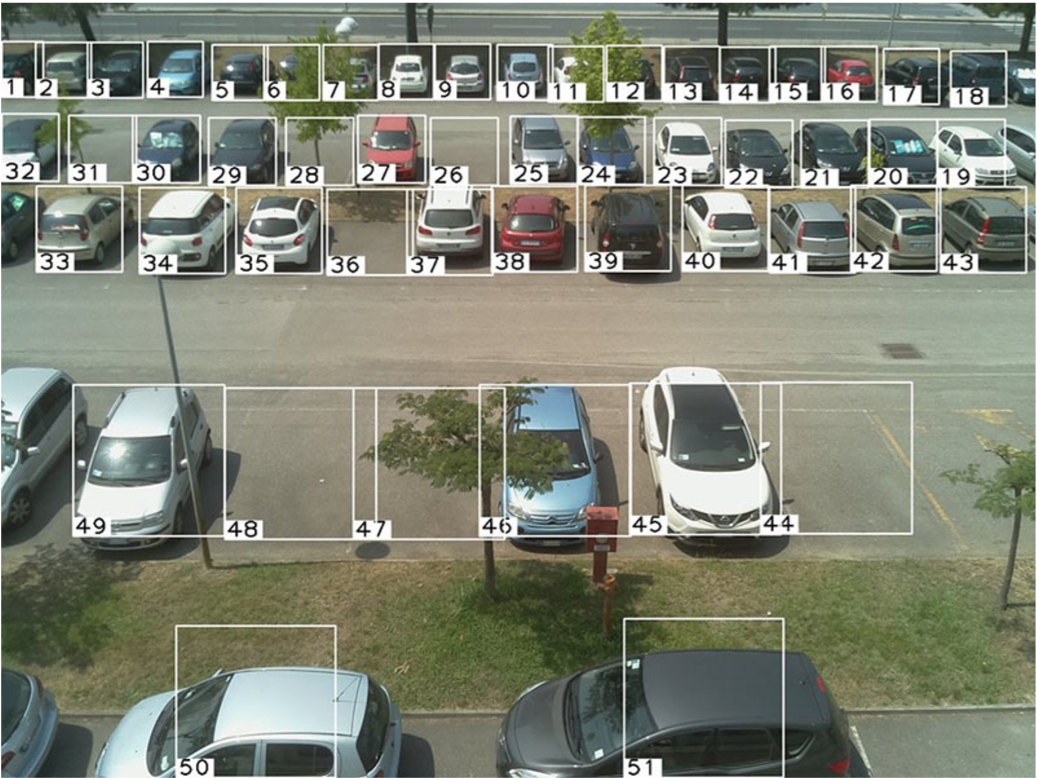
\includegraphics[width=110mm]{img/introduction/dlp_example.png}
    \centering
    \caption{Exemple d'images du corpus utilisé}
    \label{fig:dlp_example}
\end{figure} 

De la même manière, le papier \textit{Parking Stall Vacancy Indicator System Based on Deep Convolutional Neural Networks} permet d'obtenir des résultats similaires. \autocite{paper:psv}

\subsection{Détection des voitures}
Bo Li, Tianfu Wu et Song-Chun présente dans leur papier une méthode de détection de voitures à partir d'image. Ceux-ci utilisent une méthode complexe basées sur des convolutions pour détecter certaines parties des voitures (phares, portes, etc.). Sur le corpus d'images \textit{PKLot}, les résultats atteignent un taux de 55.2\% de réussite. \autocite{paper:car_detect}

\subsection{Conclusions}

En général, le problème de mesure du taux d'occupation d'un parking à l'aide de caméras vidéos est approchée à l'aide d'une segmentation des différentes places de parcs, ce qui est pertinent si les places disponibles sont toutes marquées au sol. Néanmoins, l'approche abordée dans ce travail diffère dans le but de répondre aux problèmes présentés en section \itnameref{intro.contexte} tel que les parkings sauvages. Dans cette optique, on cherchera à détecter les voitures présentes, et non pas à classifier chaque place de parc comme étant libre ou non.